\documentclass[11pt]{article}
\usepackage[T1]{fontenc}
\usepackage{lmodern,microtype,mathtools,amsthm,amssymb,booktabs,graphicx,xcolor,enumitem}
\usepackage[letterpaper,margin=0.92in,top=.85in,bottom=.86in]{geometry}
\usepackage{fancyhdr,hyperref}
\definecolor{ink}{HTML}{18324A}\definecolor{teal}{HTML}{006F6A}
\hypersetup{colorlinks=true,urlcolor=teal,linkcolor=teal,citecolor=teal,pdftitle={Six lattice rows minimize the rank-two Gram determinant asymptotically}}
\pagestyle{fancy}\fancyhf{}\fancyhead[L]{\small\sffamily\color{ink}Integral Gram determinants}\fancyhead[R]{\small\sffamily\color{ink}Rank two}\fancyfoot[C]{\small\thepage}
\setlength{\headheight}{14pt}\setlength{\emergencystretch}{2em}
\newtheorem{theorem}{Theorem}\newtheorem{lemma}[theorem]{Lemma}\newtheorem{corollary}[theorem]{Corollary}
\newcommand{\Z}{\mathbb Z}\newcommand{\R}{\mathbb R}\newcommand{\E}{\mathcal E}
\newcommand{\tp}{T_{\!*}}\newcommand{\rank}{\operatorname{rank}}
\newcommand{\sourcebase}{https://github.com/VladimirReshetnikov/ProveIt/blob/4f99495218d1a19087deabd8fb5bbb8f5df72a46/Analysis/GeneralizedRiemannHypothesis}
\begin{document}
\thispagestyle{plain}
{\sffamily\small\bfseries\color{teal} GEOMETRY OF NUMBERS}\par\vspace{6pt}
{\LARGE\bfseries\color{ink} Six lattice rows minimize the rank-two\par Gram determinant asymptotically}\par\vspace{7pt}
{\small Research note\hfill 27 November 2026}\par\vspace{10pt}
\noindent
For a two-row integer matrix with every minor nonzero, divide its Gram determinant by the square of the gcd of its minors. We determine the minimum of this integer through its quartic and cubic terms. The leading constant is an algebraic number of degree 48, determined by an explicit sum involving the first six totients. A primitive horizontal direction accounts for the cubic correction. We also determine, with bounded error, the number of columns on each row of every sufficiently large minimizer in a suitable lattice basis. The result applies unconditionally to the covolume question in ProveIt's article on Dirichlet GRH.

\section{The extremal problem}
For $A=[v_1\ \cdots\ v_n]\in\Z^{2\times n}$ with $\det(v_i,v_j)\ne0$ when $i\ne j$, set
\[
 D(A)=\gcd_{i<j}|\det(v_i,v_j)|,\qquad
 E(n)=\min_A \frac{\det(AA^{\mathsf T})}{D(A)^2}.
\]
The article's theorem on arithmetic determinant amplification gives $E(n)\ge(12/5)\binom n2$ for $n\ge5$ and attains equality at $n=5$. Its question \texttt{src:q:gram} asks for fixed-parameter minima \cite{source}. The rank-two answer for large $n$ involves the one-variable function
\begin{equation}
 F(T)=\frac{4}{3T}\sum_{1\le j\le T} w_j(1-j^2/T^2)^{3/2},\qquad
 w_j=\frac{\varphi(j)}j,\qquad T>0. \label{eq:F}
\end{equation}
The empty sum is zero. Write $C=\max_{T>0}F(T)$.

\begin{theorem}[Sharp energy and row counts]\label{th:main}
The maximum defining $C$ is attained at a unique $\tp\in(6,7)$. With $\kappa=(64C^2)^{-1}$,
\begin{equation}
 E(n)=\kappa(n-1)^4+O(n^2),\qquad
 0.068157932354<\kappa<0.068157932355.\label{eq:E}
\end{equation}
For all sufficiently large $n$, use a suitable basis of the lattice generated by the columns of any minimizing matrix. After independent sign choices, its columns consist of $(1,0)$ and primitive vectors $(m,j)$ on exactly the rows $1\le j\le6$. The number on row $j$ is
\begin{equation}
 N_j=\frac{w_j}{C\tp}\sqrt{1-j^2/\tp^2}\,(n-1)+O(1).\label{eq:Nj}
\end{equation}
The numbers $\kappa$ and $\tp^2$ generate the same degree-48 number field. All implied constants are absolute.
\end{theorem}

The weights in \eqref{eq:Nj} are approximately $0.32484,0.15610,0.19327,0.12773,0.16219,0.03587$.
For comparison, B\'ar\'any and Tokushige study the sum of the \emph{absolute} pairwise determinants in their minimum-area lattice polygon problem \cite{bt}. Kriepke and Schymura study the largest absolute minor \cite{ks}. The squared sum here admits a trace minimization that gives both a scalar optimization and its exact arithmetic profile.

\section{Normalization and change of metric}
Let $L=\sum_i\Z v_i$. Its index in $\Z^2$ is $D(A)$, by the Smith normal form, or by taking the exterior square of a generating family for $L$. In a basis of $L$ the columns generate $\Z^2$, and all determinants are divided by $D(A)$ up to a common sign. Cauchy--Binet gives
\[
 \det(AA^{\mathsf T})=\sum_{i<j}\det(v_i,v_j)^2.
\]
Consequently $E(n)$ also equals the minimum of the unnormalized squared sum over all $n$ nonparallel integer vectors. Indeed any such sum is at least its normalized value, and every normalized value occurs as an unnormalized sum in a basis of $L$. The positive integer minimum exists for each $n\ge2$. Each column of a minimizing, generating configuration is primitive. Dividing a nonprimitive vector by its content strictly decreases the squared sum.

For any positive definite $2\times2$ matrix $M$,
\begin{equation}
 \min_{g\in\mathrm{SL}_2(\R)}\operatorname{tr}(gMg^{\mathsf T})=2\sqrt{\det M}.
 \label{eq:trace}
\end{equation}
The arithmetic--geometric mean inequality proves the lower bound, and $g=(\det M)^{1/4}M^{-1/2}$ realizes it. For a lattice $\Lambda$ of covolume one, let $\mathcal P(\Lambda)$ contain one representative from each antipodal pair of primitive vectors. Formula \eqref{eq:trace}, with $M=\sum_i v_iv_i^{\mathsf T}$, gives
\begin{equation}
 2\sqrt{E(n)}=\inf_{\Lambda}\ \inf_{\substack{S\subset\mathcal P(\Lambda)\\ |S|=n}}
            \ \sum_{v\in S}|v|^2.\label{eq:min}
\end{equation}
All $n\ge2$ distinct directions span. In a fixed lattice the inner minimum selects its $n$ shortest primitive directions, with any choice at a tie. An isotropized minimizing matrix realizes the joint infimum.

\section{Counting primitive directions in a disk}
Define the truncated sum and count
\[
 P_\Lambda(R)=\sum_{v\in\mathcal P(\Lambda)}(R^2-|v|^2)_+,
 \qquad N_\Lambda(R)=\#\{v\in\mathcal P(\Lambda):|v|\le R\}.
\]
A reduced basis, after rotation, has the form $(a,0),(a\theta,1/a)$ with $a$ the shortest nonzero length and $|\theta|\le1/2$. The first vector is primitive and extends to a lattice basis. Reducing the other vector modulo the first gives $a^2\le a^2/4+a^{-2}$, so $a\le(4/3)^{1/4}$. Choose the positive representative on each nonhorizontal pair. Then row $j>0$ consists of $(a(m+j\theta),j/a)$ with $m\in\Z$ and $\gcd(m,j)=1$. Row zero has a single representative. The natural parameter is $T=aR$.

\begin{lemma}[Two precisions for the truncated sum]\label{lem:count}
Uniformly in the lattice, as $R\to\infty$,
\begin{equation}
 P_\Lambda(R)=R^4 F(T)+O\bigl(R^3\log(2R)\bigr).\label{eq:crude}
\end{equation}
For any fixed compact interval $I\subset(0,\infty)$, uniformly for $T\in I$,
\begin{align}
 P_\Lambda(R)&=R^4F(T)+R^2+O_I(1),\label{eq:sharp}\\
 N_\Lambda(R)&=R^2 B(T)+1+O_I(1),\qquad
 B(T)=\frac2T\sum_{1\le j\le T}w_j\sqrt{1-j^2/T^2}.
 \label{eq:count}
\end{align}
In particular $B(T)=2F(T)+(T/2)F'(T)$.
\end{lemma}
\begin{proof}
For $1\le j\le T$ put $h=(R^2-j^2/a^2)^{1/2}$. In the horizontal coordinate the summand is $f(x)=(h^2-x^2)_+$. The integral of $f$ is $4h^3/3$. The mean density of coprime indices in the row is $w_j/a$, so the sum of the integral terms is $R^4F(T)$.

For the uniform error use $\mathbf1_{(m,j)=1}=\sum_{d\mid(m,j)}\mu(d)$. On a shifted grid of spacing $ad$, the error between the sum of $f$ and the integral divided by $ad$ is at most the total variation $2h^2$, by comparison on consecutive cells. Thus the row error is $O(R^2\tau(j))$, where $\tau$ counts divisors. Since $\sum_{j\le T}\tau(j)\le T(1+\log T)$ for $T\ge1$ and $T=O(R)$, summing and adding the horizontal contribution proves \eqref{eq:crude}, also for $T<1$.

For the finer error, a shifted grid with spacing $d_0$ satisfies
\[
 \left|\sum_{k\in\Z} f(d_0 k+u)-d_0^{-1}\int f\right|
 \le d_0\,\operatorname{Var}(f').
\]
Indeed integrate the linear interpolant on each cell. Its slope is the average of $f'$ there, so the integral error on a cell is at most $d_0^2$ times the variation of $f'$ on the cell; jumps at boundaries are harmless with one-sided representatives. Equivalently the same bound follows first for smooth $f$ and then by mollification. Here $\operatorname{Var}(f')=8h$. Split the row into the $\varphi(j)$ primitive residue classes modulo $j$ and take $d_0=aj$. Only boundedly many rows and residue classes occur, and $aR=T$ is bounded. The total error on positive rows is $O_I(1)$. The horizontal point contributes $R^2-a^2=R^2+O_I(1)$. Counting points on each residue grid in $[-h,h]$ gives its length divided by $aj$ with $O(1)$ error, proving \eqref{eq:count}. Direct differentiation proves the identity for $B$, including at integers by continuity.
\end{proof}

\section{The certified scalar maximum}
\begin{lemma}\label{lem:max}
The maximum of $F$ occurs at the unique $\tp\in[6.15,6.60]$ satisfying
\begin{equation}
 \sum_{j=1}^6 w_j(4j^2-\tp^2)\sqrt{\tp^2-j^2}=0. \label{eq:root}
\end{equation}
It is nondegenerate. The intervals below have rational decimal endpoints:
\[
 \begin{split}
 6.349265427728&<\tp<6.349265427729,\\
 0.478797428690&<C<0.478797428691.
 \end{split}
\]
Outside $[6.15,6.60]$ one has $F(T)<0.4787$.
\end{lemma}
\begin{proof}
Let $A_0(x)=\sum_{j\le x}\varphi(j)/j$. M\"obius inversion gives
$A_0(x)=\sum_{d\le x}\mu(d)\lfloor x/d\rfloor/d$.
Comparison with $x\sum_{d\ge1}\mu(d)/d^2=6x/\pi^2$, bounding the floor errors by the harmonic sum and the tail by $x/\lfloor x\rfloor$, gives $|A_0(x)-6x/\pi^2|\le\log x+3$ for $x\ge1$. For $x<1$ the error is at most one. Partial summation against $(1-(x/T)^2)^{3/2}$, whose integral on $[0,T]$ is $3\pi T/16$ and whose total decrease is one, gives
\[
 \left|F(T)-\frac{3}{2\pi}\right|\le \frac{4(\log T+3)}{3T}\qquad(T\ge1).
\]
For $T\ge20000$ the upper bound is below $0.4787$. The following two finite checks close the remaining ranges. Their executable proof is \texttt{verify\_constant.py}; all rounding uses integers.
\begin{enumerate}[leftmargin=*,itemsep=2pt]
\item For $1\le j\le20000$ the totient sieve and upper rounding of each $10^9 w_j$ certify $A_0(j)\le 76j/125+3/5$. This also holds between integers by monotonicity of the right side. For $1000\le T\le20000$ partial summation gives $F(T)\le(76/125)\pi/4+4/(5T)<0.4787$.
\item On $[1,1000]\setminus(6.15,6.60)$ subdivide into intervals $[l,r]$. The summands of $TF(T)$ are nondecreasing, hence $F(T)\le r F(r)/l$. Round each radical upwards by integer square root, and bisect any interval whose bound exceeds or equals $0.4787$. All $3255$ terminal intervals pass. Below $1$ the sum vanishes.
\end{enumerate}
A lower evaluation gives $F(6.35)>0.47879$. With $u=T^2$ the derivative of $F$ on $(6,7)$ has the sign of $G(u)=\sum_{j=1}^6w_j(4j^2-u)\sqrt{u-j^2}$. Its second derivative is
\[
 G''(u)=-\frac{3u}{4}\sum_{j=1}^6w_j(u-j^2)^{-3/2}<0 .
\]
At $u=6.15^2$ and $6.60^2$ the signs are respectively positive and negative, certified by the same rational radical bounds. Strict concavity gives a unique crossing with strictly negative derivative, hence $F''(\tp)<0$. Bisection and the monotone bound $F(T)\le rF(r)/l$ give the displayed intervals and \eqref{eq:E}'s interval for $\kappa$.
\end{proof}

\section{The minimum and the six rows}
For every $S$ of $n$ directions in $\Lambda$ one has
\begin{equation}
 \sum_{v\in S}|v|^2\ \ge\ nR^2-P_\Lambda(R).
 \label{eq:duality}
\end{equation}
Take $R^2=(n-1)/(2C)$. On $I=[6.15,6.60]$ formula \eqref{eq:sharp} gives $P_\Lambda(R)\le CR^4+R^2+O(1)$. Outside $I$ the uniform bound \eqref{eq:crude} has an error $o(R^4)$, absorbed for large $R$ by the fixed gap $C-0.4787>0$. Thus \eqref{eq:min} and \eqref{eq:duality} yield
\begin{equation}
 2\sqrt{E(n)}\ \ge\ (n-1)R^2-CR^4-O(1)
       =\frac{(n-1)^2}{4C}-O(1). \label{eq:low}
\end{equation}

For the matching upper bound take $a=\tp/R$ and the rectangular lattice generated by $(a,0),(0,1/a)$. For large $n$, $a$ is its shortest length. Since $F'(\tp)=0$, Lemma~\ref{lem:count} gives $N_\Lambda(R)=1+2CR^2+O(1)=n+O(1)$. On row one the boundary in the integer coordinate is $m_0=(R/a)\sqrt{1-\tp^{-2}}$. Moving $m$ a bounded number of steps past $m_0$ in either direction changes $a^2m^2+a^{-2}$ by $O(1)$, since $aR=\tp$. There are enough such distinct directions to correct the $O(1)$ discrepancy with each selected or discarded point within $O(1)$ of squared radius $R^2$. For the resulting set $S$,
\[
 \sum_{v\in S}|v|^2=nR^2-P_\Lambda(R)+O(1)
                  =\frac{(n-1)^2}{4C}+O(1).
\]
Together with \eqref{eq:low} this proves $\sqrt{E(n)}=(n-1)^2/(8C)+O(1)$, and squaring gives \eqref{eq:E}.

To prove the structural assertion, isotropize a minimizing configuration via \eqref{eq:trace}. Its exact sum of squared lengths is $2\sqrt{E(n)}$. The fixed gap in Lemma~\ref{lem:max} and \eqref{eq:crude} force $T\in I$ for large $n$. The upper bound just obtained and \eqref{eq:duality} with \eqref{eq:sharp} now imply $R^4(C-F(T))=O(1)$. By uniqueness and $F''(\tp)<0$,
\begin{equation}
                    T=\tp+O(R^{-2}).
\end{equation}
The nonnegative slack in \eqref{eq:duality} is $O(1)$. More explicitly, it is the sum of $R^2-|v|^2$ over omitted interior points and $|v|^2-R^2$ over selected exterior points. Thus every point with squared length below $R^2-O(1)$ is selected, and none above $R^2+O(1)$ is selected, with a common absolute constant. The unique horizontal representative is selected, and rows $j\ge7$ are excluded since $7/\tp>1$. Each of rows $1,\ldots,6$ meets the boundary away from a tangent. Increasing the squared radius by a bounded amount changes its horizontal half-width in \emph{integer coordinates} by $O(1)$, uniformly in the shear $\theta$. The elementary interval count on row $j$ therefore gives
\[
 N_j=\frac{2w_jR^2}{T}\sqrt{1-j^2/T^2}+O(1).
\]
Replacing $T$ by $\tp$ costs $O(1)$ and gives \eqref{eq:Nj}. Every coefficient there is positive. This completes the proof of Theorem~\ref{th:main}.

\begin{figure}[ht]
\centering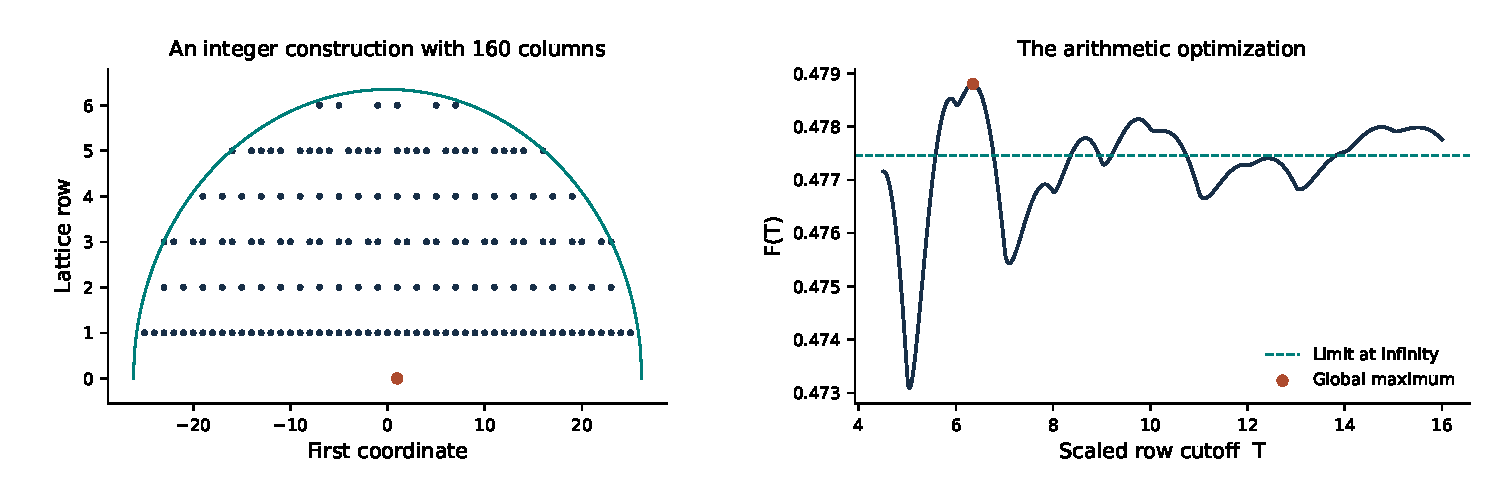
\includegraphics[width=.98\linewidth]{six_rows.pdf}
\caption{A finite construction in integer coordinates, and the profile in \eqref{eq:F}. The separate point on row zero contributes the shift from $n$ to $n-1$. The dashed line is $3/(2\pi)$. The global maximum is certified in Lemma~\ref{lem:max}.}
\end{figure}

\section{Algebraic degrees of the extremal constants}

\begin{theorem}\label{th:degree}
The field $K=\mathbb Q(\tp^2)$ has degree $48$ and equals
$\mathbb Q(\kappa)$. Each of $\tp$ and $C$ has degree $96$ over $\mathbb Q$.
\end{theorem}

\begin{proof}
Set $u=\tp^2$ and $b_j=30w_j$ for $1\le j\le6$, so
$(b_1,\ldots,b_6)=(30,15,20,15,24,10)$. Introduce two
parameters $s,t$ and put
\[
 B_j=\bigl(b_j(4j^2-x)+s\,\mathbf1_{j=1}
              +t b_j(x-j^2)\bigr)\sqrt{x-j^2}.
\]
Write $\Omega(x,s,t)$ for the product of $B_1+\sum_{j=2}^6\varepsilon_j B_j$
over the $32$ choices of signs. Changing any radical sign preserves the product.
For the first sign change, negate all $32$ factors and permute them. Applying
this argument with independent formal radicals shows that each radical has
even exponent. Thus $\Omega\in\Z[x,s,t]$ and its degree in $x$ is at most $48$.
Set $P(x)=\Omega(x,0,0)$, and let $H_s,H_t$ be the two parameter derivatives
at $s=t=0$. On the positive branch at $x=u$ the all-plus factor vanishes by
the critical-point equation for $F$. In particular $P(u)=0$.

The accompanying exact certificate gives $\deg(P\bmod 53)=48$ and shows
that this reduction is irreducible. Here are the details of the calculation
for independent reproduction. Evaluate the three polynomials $P,H_s,H_t$ at
$x=0,\ldots,48$ over $\mathbb F_{53}$ and interpolate. To compute a product
over signs, successively multiply by its conjugate under each of the last
five radical sign changes. In the basis indexed by subsets $I\subseteq
\{1,\ldots,6\}$, multiplication replaces the two subsets $I,J$ by
$I\mathbin\triangle J$ and contributes a factor
$\prod_{j\in I\cap J}(x-j^2)$. The product rule carries both derivatives.
In $\mathbb F_{53}[X]$, writing $\bar P$ for the reduction, the certificate
checks
\[
 X^{53^{48}}\equiv X\pmod{\bar P},\qquad
 \gcd(\bar P,X^{53^d}-X)=1\quad(d=16,24).
\]
Since $2,3$ are the prime divisors of $48$, these tests exclude every
proper possible irreducible-factor degree and prove irreducibility. Gauss's
lemma now gives $[K:\mathbb Q]=48$.

The root $u$ of $P$ is simple. Every radical is analytic near this real
point, so exactly one sign factor vanishes. Differentiating the product
and cancelling the nonvanishing factors gives
\[
 \frac{H_t(u)}{H_s(u)}
 =\frac{\sum_{j=1}^6 b_j(u-j^2)^{3/2}}{\sqrt{u-1}},
 \qquad
 \kappa=\frac{2025u^4 H_s(u)^2}{256(u-1)H_t(u)^2}.
\]
Both derivatives at $u$ are nonzero. This places $\kappa$ in $K$.
In $\mathbb F_{53}[X]/(\bar P)$, the denominator of the formula is
nonzero. The certificate verifies by cross multiplication that neither
the $16$th nor the $24$th iterate of Frobenius fixes the quotient.
It therefore has degree $48$ over $\mathbb F_{53}$. To justify reduction,
the leading coefficient of $P$ is a $53$-adic unit. After dividing by it,
$P$ is monic over $\Z_{(53)}$, so reduction of $\Z_{(53)}[u]$
gives the stated finite field. The map extends upon inverting the displayed
denominator. Any rational polynomial relation on $\kappa$ can be scaled to
a primitive integer relation, whose reduction is a nonzero polynomial
annihilating the finite-field quotient. Consequently $\kappa$ has degree
at least $48$, proving $\mathbb Q(\kappa)=K$.

Finally let $L$ be the leading coefficient of $P$. Since its degree is even,
the norms of $u$ and $u-1$ are $P(0)/L$ and $P(1)/L$. The certificate
gives their residues $50\pmod {53}$ and $42\pmod {59}$, respectively,
both quadratic nonresidues at primes where $L$ is a unit. Neither norm is
a rational square, hence neither $u$ nor $u-1$ is a square in $K$.
Now $\tp=\sqrt u$, and
$C=2H_t(u)\sqrt{u-1}/(45u^2 H_s(u))$. Since $\mathbb Q(C)$ contains
$\kappa$, it contains $K$. Both claimed quadratic extensions follow.
\end{proof}


\section{Higher ranks and numerical witnesses}
Let $E_r(n)$ denote the analogous minimum for an integer $r\times n$ matrix with every maximal minor nonzero, normalized by the square of their gcd.
\begin{corollary}[Contraction and duality]
For $2\le r\le n-2$,
\[
 \frac{E_r(n)}{\binom nr}\ \ge \max\!\left\{\frac{E(n-r+2)}{\binom{n-r+2}{2}},\,
                   \frac{E(r+2)}{\binom{r+2}{2}}\right\},\qquad E_{n-2}(n)=E(n).
\]
\end{corollary}
\begin{proof}
Freeze $r-2$ column indices $I$. A unimodular row operation carries the rational span of those columns to the first $r-2$ coordinate axes, by choosing a basis of its saturated lattice. Each minor extending $I$ is, up to sign, a common nonzero integer times a two-row minor of the projected columns. Dividing this local family by its own gcd gives normalized rank-two minors. The global gcd divides this local gcd, so the sum of squared globally normalized minors extending $I$ is at least $E(n-r+2)$. Each full minor occurs $\binom r2$ times in the sum over $I$. Divide by the number of incidences to get the first bound. The Hodge star of the primitive exterior product of a basis of the saturated rational row space is the primitive exterior product of its orthogonal complement, up to sign: it spans the required exterior line over $\mathbb Q$, and taking signed complementary coordinates preserves primitivity. Thus $E_r(n)=E_{n-r}(n)$. Apply the first bound again.
\end{proof}
For fixed $r$ the corollary gives at least $(2\kappa+o(1))n^2\binom nr$. Determining the sharp constant or even the correct general order for fixed $r\ge3$ remains open here.

\begin{center}
\begin{tabular}{rrr}\toprule
Columns & Squared sum for the constructed matrix & Squared sum divided by $(n-1)^4$\\\midrule
100 & $6\,546\,225$ & 0.068147535\\
1\,000 & $67\,885\,760\,907$ & 0.068157984\\
10\,000 & $681\,306\,789\,878\,949$ & 0.068157938\\\bottomrule
\end{tabular}
\end{center}
The witnesses use rational parameters close to $C,\tp$ for exact comparison of squared lengths. The columns include $(1,0)$ and a point on row one, so their index is one. The table gives upper bounds at finite $n$. The lower bound in Theorem~\ref{th:main} comes from the uniform estimates on all lattices.

\paragraph{Further questions.}
Determine the limit points of $(E(n)-\kappa(n-1)^4)/n^2$. The row endpoints and the basis shear enter at this scale. For a fixed number of zero minors, one must also optimize the multiplicities on repeated directions. A finite classification of all minimizing matrices, including the first $n$ at which six rows are forced, would require explicit error constants in the rigidity argument.

\begin{thebibliography}{9}
\bibitem{source} V. Reshetnikov, \emph{ProveIt}, \href{\sourcebase/Article/sections/src.tex}{Article, section on integral Gram determinants}, theorem \texttt{src:thm:gram} and question \texttt{src:q:gram}, commit \texttt{4f99495218d1}, 27 November 2026. See also the \href{\sourcebase/README.md}{project overview}.
\bibitem{bt} I. B\'ar\'any and N. Tokushige, \href{https://www.renyi.hu/~barany/cikkek/94.pdf}{The minimum area of convex lattice $n$-gons}, \emph{Combinatorica} \textbf{24} (2004), 171--185.
\bibitem{ks} B. Kriepke and M. Schymura, \href{https://arxiv.org/abs/2502.15394}{On generic $\Delta$-modular integer matrices with two rows}, arXiv:2502.15394.
\end{thebibliography}
\end{document}
